% Appendix B

\chapter{Simulated Annealing} % Main appendix title

This appendix justifies the name of the quantum approach we use in the present work -- \textit{Quantum Annealing} (QA) -- to solve \textit{Quadratic Unconstrained Binary Optimization} (QUBO) problems, see Chapter\,\ref{Chapter2}. In the next sections, we show that the expressions we get in the classical approach known as \textit{Simulated Annealing} (SA), have the same functional form as the ones we get with QA\,\cite{Kadowaki1998QuantumModel}. To do that we are going to develop the solution for a stochastic problem. For a better understanding about stochastic problems, see Refs.\,\cite{Schneider2006StochasticOptimization} and \cite{AlvaroDiazComputacionAdiabatica}. 
\label{AppendixB} % For referencing this appendix elsewhere, use \ref{AppendixB}
%%%%%%%%%%%%%%%%%%%%%%%%%%%%%%%%%%%%%%%%%%%%%%%%%%%%%%%%%%%%%%%%%%%%%%%%%%%%%%%%%%%%%%%%%%%%%%%%%%%%%%%%%%
%     B.1 MASTER EQUATION
%%%%%%%%%%%%%%%%%%%%%%%%%%%%%%%%%%%%%%%%%%%%%%%%%%%%%%%%%%%%%%%%%%%%%%%%%%%%%%%%%%%%%%%%%%%%%%%%%%%%%%%%%%
\section{Master Equation}
A master equation is used to characterize the time-evolution of a given system that switches between states according to a transition rate for a given distribution. These switches between states are going to generate a new configuration that would be chosen as the current configuration if the energy difference between the current configuration and the new one is negative, $\Delta E = E_{\text{new}} - E_{\text{current}} < 0$. However, if $\Delta E > 0$, there is still a possibility for the new configuration to be chosen given by a probability distribution $P \left(\Delta E, T \right)$ that depends on the energy difference and the temperature $T$ of the system.
\subsection{Discrete Processes}
Suppose we have a space of states $\Gamma = \{\uparrow \uparrow,\downarrow \uparrow,\uparrow \downarrow,\downarrow \downarrow \} \equiv \{1, 2, 3, 4 \}$ and a discrete stochastic process, e.g., $\{X_{t}, t= 0,1,2,...\} \rightarrow \{1,4,2,3,1,..\}$. Furthermore, assume that the actual setting of our system only depends on the previous one, i.e., the probability of being in state \textit{j} at time $t+1$, $X_{t+1}= j$, given that the current state is \textit{i}, $X_{t} = i$, does not depend on previous configurations. Mathematically,
\begin{equation}
\label{eq: MarkovChain}
    P\left(X_{t+1} = j | X_{t} = i\right) = P\left(X_{t+1}=j | X_{t} = i, X_{t-1} =i_{t-1},...,X_{0} = i_{0}\right)\ .
\end{equation}
The equation Eq.\,\eqref{eq: MarkovChain} is known as \textbf{Markov chain} condition and the conditional probabilities are named \textit{transition probabilities}.\\
The normalization condition for probabilities is also fulfilled, i.e., starting from a state  \textit{i} any state \textit{j} -- where \textit{j} can be also the current state -- has a transition probability such that
\begin{equation}
    \sum_{j}P\left(X_{t+1} = j | X_{t} = i\right) = 1, \;\; \forall i\ .
\end{equation}
\begin{theorem}{Total Probability}{}
Consider an event $A$ in a discrete set of events $\{B_{i}\}$, the probability of occurrence of event $A$ is given by,
\begin{equation}
    P\left(A\right) = \sum_{i}P\left(A|B_{i}\right)P\left(B_{i}\right)\ ,
\end{equation}
where $P\left(A|B_{i}\right)$ is the probability of occurrence of event $A$ given that event $B_{i}$ has already happened. 
\end{theorem}
Renaming variables,
\begin{align}
    \label{eq:Renaming1}
    \Pi_{i}(t) \equiv P\left(X_{t} = i\right) \\
    \label{eq:Renaming2}
    p_{i \leftarrow j} \equiv P\left(X_{t+1} = i | X_{t}=j\right)\ .
\end{align}
From equations Eq.\,\eqref{eq:Renaming1} and Eq.\,\eqref{eq:Renaming2}, we can write,
\begin{align}
        \Pi_{i}(t+1) &= p_{i \leftarrow i}\Pi_{i}(t) + \sum_{j \neq i} p_{i \leftarrow j}\Pi_{j}(t) \\ 
        p_{i \leftarrow i} &= 1 - \sum_{j\neq i}p_{j \leftarrow i}\ .
\end{align}
Combining the last two equations,
\begin{align}
    \Pi_{i}(t+1) &= \left[1 - \sum_{j\neq i}p_{j \leftarrow i}\right]\Pi_{i}(t) + \sum_{j\neq i}p_{i \leftarrow j}\Pi_{j}(t),\\
    \Pi_{i}(t+1) - \Pi_{i}(t) &= -\Pi_{i}(t) \sum_{j \neq i}p_{i \leftarrow j} + \sum_{j \neq i} p_{i \leftarrow j}\Pi_{j}(t), \\
    \label{eq: MasterEquationDiscrete}
    d\Pi_{i}(t) \equiv \Pi_{i}(t+1) - \Pi_{i}(t) &=  -\Pi_{i}(t) \sum_{j \neq i}p_{i \leftarrow j} + \sum_{j \neq i} p_{i \leftarrow j}\Pi_{j}(t)\ .
\end{align}
we get the master equation of a Markov stochastic discrete process.
\subsection{Continuous Processes}
In the case where we deal with a continuous process\footnote{In this thesis, a continuous process is understood as a stochastic process that is continuous in time but whose state space is discrete.} we need  to work with transition rates defined by
\begin{equation}
    \mathcal{L}_{i \leftarrow j} = 
    \begin{cases}
    \mathcal{L}_{i \leftarrow j} \;\; i\neq j\\
    -\sum_{k\neq i}\mathcal{L}_{k \leftarrow i} \;\; i = j\ ,
    \end{cases}
\end{equation}
so that the master equation can be written as
\begin{equation}
\label{eq: MasterEquationContinuous}
    \frac{d\Pi_{i}(t)}{dt} = \sum_{j}\mathcal{L}_{i \leftarrow j} \Pi_{j}(t)\ .
\end{equation}
If we know $\Pi_{i}(t_{0})$ we can know the probability at later times. Assume our system has reached the steady state, i.e., $d\Pi_{i}/dt = 0$, which implies
\begin{equation}
\label{eq: StationaryCondition}
    \Pi_{i}^{\mathrm{eq}} \sum_{j\neq i} \mathcal{L}_{j \leftarrow i} = \sum_{j \neq i}\mathcal{L}_{i \leftarrow j}\Pi_{j}^{\mathrm{eq}}\ .
\end{equation}
A sufficient but not necessary condition to fulfill Eq.\,\eqref{eq: StationaryCondition} is,
\begin{equation}
    \Pi_{i}^{\mathrm{eq}}\mathcal{L}_{j \leftarrow i} = \mathcal{L}_{i \leftarrow j}\Pi_{j}^{\mathrm{eq}}\ , 
\end{equation}
which is known as the \textbf{detailed balanced condition}.\\
The evolution of our system is determined by knowing an initial state and the transition rate expression. Metropolis \textit{et al.}\,\cite{Metropolis1953}, in connection to statistical mechanics, chose the Boltzmann distribution
\begin{equation}
    \Pi_{i}^{\mathrm{eq}} = \frac{1}{Z}\exp\left(- \frac{\mathcal{H}_{i}}{k_{B}T}\right), \;\;\; Z = \sum_{i}\exp\left(-\frac{\mathcal{H}_{i}}{k_{B}T}\right)\ ,
\end{equation}
which implies,
\begin{equation}
    \frac{\mathcal{L}_{j \leftarrow i}}{\mathcal{L}_{i \leftarrow j}} = \exp\left(\frac{\mathcal{H}_{i} - \mathcal{H}_{j}}{k_{B}T}\right)\ .
\end{equation}
The last expression does not define uniquely the transition rate so we need a criterion for that. There are two common criteria:
\begin{itemize}
    \item\textbf{Metropolis criterion:} $\mathcal{L}_{j \leftarrow i} = \min \left[1,\exp\left(\mathcal{H}_{i}-\mathcal{H}_{j}/\left(k_{B}T\right)\right)\right]$. This condition guarantees a transition into states with lower energy without forbidding a transition to higher energy states, where this transition rate depends on the energy difference. 
    \item \textbf{Heat bath criterion:} $\mathcal{L}_{i \leftarrow j} = \frac{\Pi_{j}^{\mathrm{eq}}}{\Pi_{i}^{\mathrm{eq}} + \Pi_{j}^{\mathrm{eq}}} = \left[1 + \exp\left(\frac{\mathcal{H}_{j}- \mathcal{H}_{i}}{k_{B}T}\right)^{-1}\right]$. 
\end{itemize}
 The transition rates do not guarantee the optimal value of our objective function. Hereafter, we will consider $k_B = 1$.
\subsection{Annealing Schedules}
The annealing approach considers a temperature that starts from a high value and decreases gradually with time. The dependence of temperature with respect to time $t$ is named annealing schedule. There are many annealing schedules but the most common ones are:
\begin{itemize}
    \item \textbf{Geman-Geman:} guarantees that the absolute minimum is reached when $t\to\infty$\,\cite{Geman1984StochasticImages}. It is given by
    \begin{equation}
        T(t) = \frac{a}{b + \log{t}}\ .
    \end{equation}
\end{itemize}
Since we do not have infinite time to perform our simulations, we need schedules that are faster despite their not guaranteeing convergence to the global minimum. 
\begin{itemize}
    \item \textbf{Linear cooling:} $T(t) = a - bT$ where $a = T_{0}$ -- initial temperature -- and $b \in (0.01,0.2)$.
    \item \textbf{Exponential cooling:} $T(t) = ab^{t}$ where $a = T_{0}$ -- initial temperature -- and $b \in (0.8,0.999)$.
\end{itemize}

%%%%%%%%%%%%%%%%%%%%%%%%%%%%%%%%%%%%%%%%%%%%%%%%%%%%%%%%%%%%%%%%%%%%%%%%%%%%%%%%%%%%%%%%%%%%%%%%%%%%%%%%%%
%     B.2 TSP Example
%%%%%%%%%%%%%%%%%%%%%%%%%%%%%%%%%%%%%%%%%%%%%%%%%%%%%%%%%%%%%%%%%%%%%%%%%%%%%%%%%%%%%%%%%%%%%%%%%%%%%%%%%%
\section{Traveling Salesman Problem}
The traveling salesman problem (TSP) is an NP-hard combinatorial optimization problem. That means it does not have a polynomial-time solution. The goal of our traveling salesman is to find the shortest path to visit all the $n$ regions in a given list $R$, which are represented by nodes in a graph, by annotating the position $P$ that each region has in the path, returning to the initial region. The distance between nodes $u,v \in R$, $D(u,v)$, measured in units of length, is calculated using the Euclidean metric
\begin{equation}
    D(u,v) \equiv D_{uv}= \sqrt{\left|x_{v} - x_{u}\right|^{2} + \left|y_{v} - y_{u} \right|^{2}}\ . 
\end{equation}
The objective function to minimize for a graph with $n$ nodes can be written as
\begin{equation}
\label{eq:TSP_noconstraints}
    \min_{\vec{x}} f(\vec{x}) = \min_{\vec{x}} \sum_{v} \sum_{u} \sum_{i=0}^{i<n}D_{u,v}x_{v,i}x_{u, i+1}\ ,
\end{equation}
where the coefficients $x_{v,i}$ are binary variables that indicate if node $v \in R$ is in the position $i\in P$ of the tour, represented by the vector $\mathbf{x}$. Furthermore the distance between nodes is symmetric $D_{uv} = D_{vu}$ which is taken into account when creating the matrix $D_{uv}$.
%%%%%%%%%%%%%%%%%%%%%%%%%%%%%%%%%%%%%%%%%%%%%%%%%%%%%%%%%%%%%%%%%%%%%%%%%%%%%%%%%%%%%%%%%%%%%%%%%%%%%%%%%%
%     B.2.1 Constraints
%%%%%%%%%%%%%%%%%%%%%%%%%%%%%%%%%%%%%%%%%%%%%%%%%%%%%%%%%%%%%%%%%%%%%%%%%%%%%%%%%%%%%%%%%%%%%%%%%%%%%%%%%%
\subsection{Constraints}
The traveling salesman has to visit each node just once in the whole path
\begin{equation}
    \sum_{i=0}^{i<n}x_{u,i} = 1 \quad  \forall \; u \in R\ ,
\end{equation}
and each stop of the tour has one node
\begin{equation}
    \sum_{u}x_{u, i} = 1 \quad  \forall \; i \in P\ .
\end{equation}
The constraints can be taken into account in the cost function by using the Lagrange multipliers $\{\lambda_{i}\}_{i \in P}$ and $\{\lambda_{u}\}_{u \in R}$
\begin{align}
        \label{eq: ObjectiveMatrixFunction}
    \begin{split}
   \min_{\vec{x}} f(\vec{x}) = \min_{\vec{x}} \sum_{v} \sum_{u} \sum_{i=0}^{i<n}D_{u,v}x_{v,i}x_{u, i+1}\\
   - \sum_{i=0}^{i<n}\lambda_{i}\left(\sum_{u} x_{u, i} - 1\right)^{2} - \sum_{u}\lambda_{u} \left( \sum_{i=0}^{i<n}x_{u,i} - 1\right)^{2}\ .
\end{split}
\end{align}
The problem can be re-written to have the functional form of a QUBO problem $\min_{x}x^{T}Qx$, where $Q$ is a matrix that stores the Hamiltonian coefficients. For this particular problem it is necessary to map the two indices of our binary variables $x_{u,i}$ into a single index, see Ref. \cite{Jain2021SolvingComputer}.
If the constraints are taken into account in the loops of our program, then the function to minimize is just Eq.\,\eqref{eq:TSP_noconstraints} which produces Figure\,\ref{fig:TSP_SA}.
\begin{figure}[H]
    \centering
    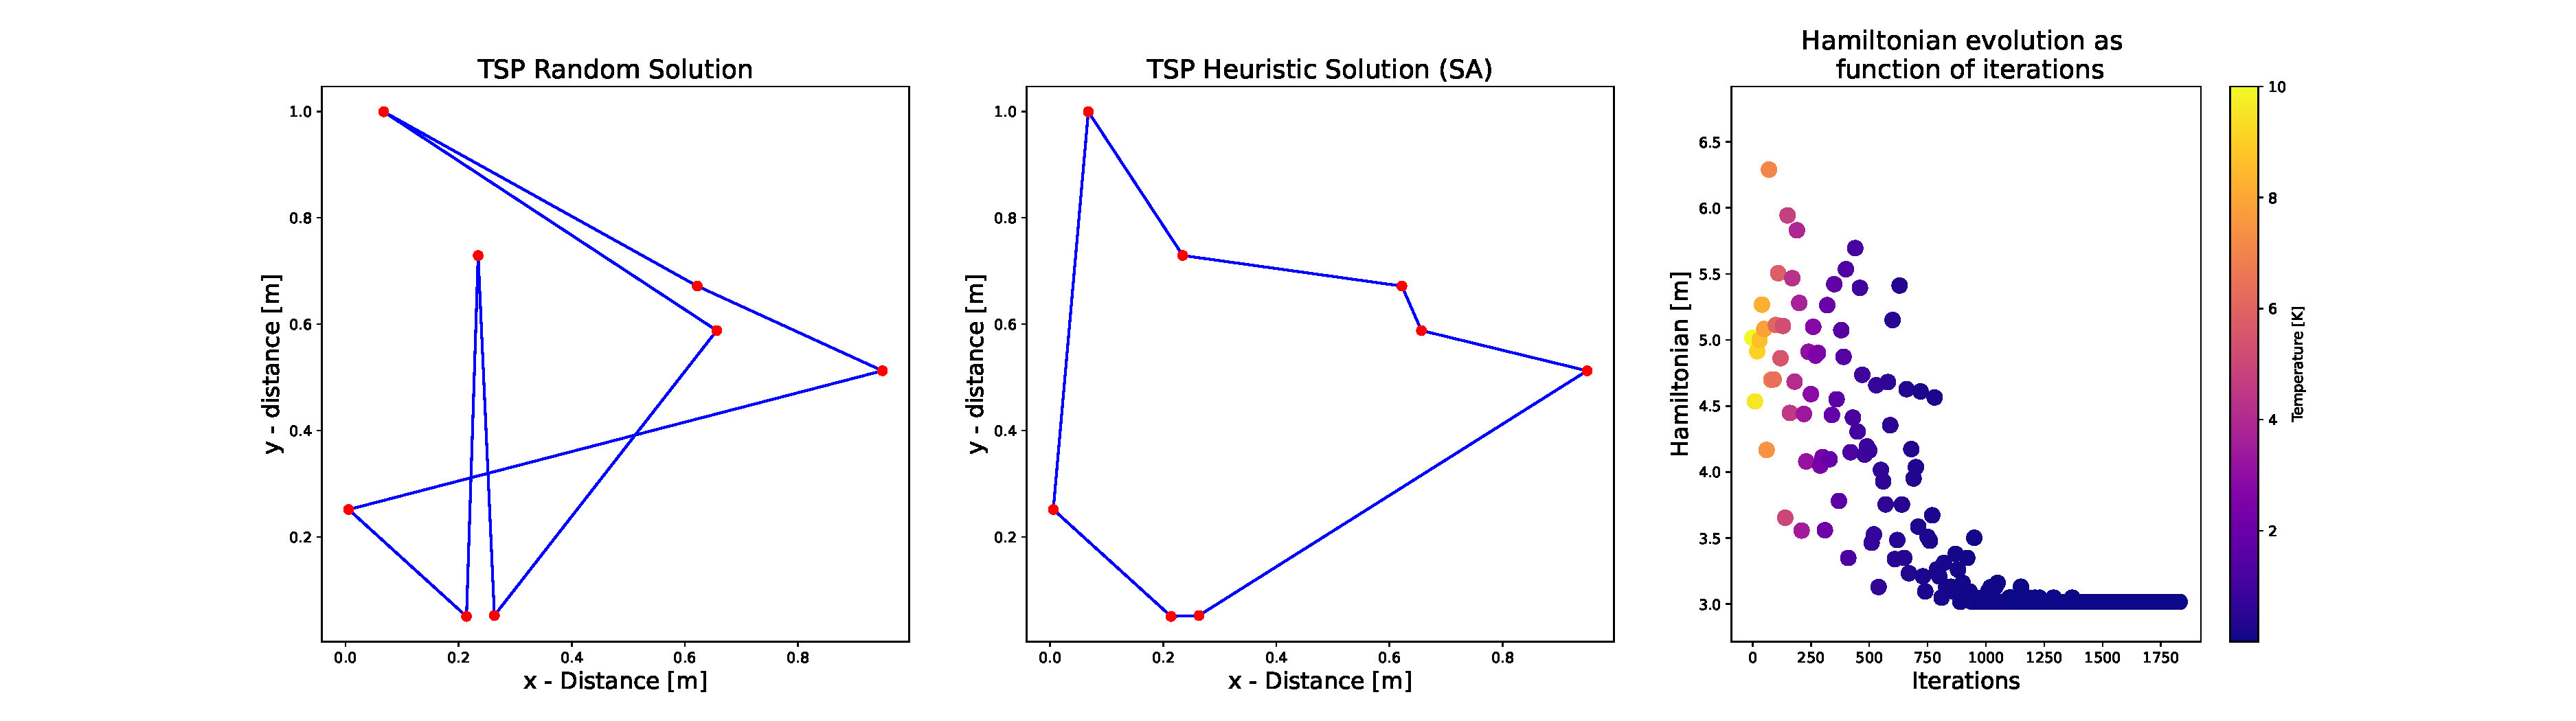
\includegraphics[width=\textwidth]{Figures/TSP_SA.pdf}
    \caption{Simulated annealing process for a 20-nodes travelling salesman problem, where nodes are represented by black dots. The code to produce the figure can be found in Appendix\,\ref{AppendixD}.\textbf{ Left:} Plot showing a random path (red) to travel the nodes and the path (blue) obtained for an instance of simulated annealing. \textbf{Right:} Hamiltonian as a function of iterations and temperature.}
    \label{fig:TSP_SA}
\end{figure}

